\documentclass[%
 reprint,
%superscriptaddress,
%groupedaddress,
%unsortedaddress,
%runinaddress,
%frontmatterverbose, 
%preprint,
%showpacs,preprintnumbers,
%nofootinbib,
%nobibnotes,
%bibnotes,
 amsmath,amssymb,
 aps,
%pra,
%prb,
%rmp,
%prstab,
%prstper,
%floatfix,
]{revtex4-1}

\usepackage{graphicx}% Include figure files
\usepackage{dcolumn}% Align table columns on decimal point
\usepackage{bm}% bold math
%\usepackage{hyperref}% add hypertext capabilities
%\usepackage[mathlines]{lineno}% Enable numbering of text and display math
%\linenumbers\relax % Commence numbering lines

%\usepackage[showframe,%Uncomment any one of the following lines to test 
%%scale=0.7, marginratio={1:1, 2:3}, ignoreall,% default settings
%%text={7in,10in},centering,
%%margin=1.5in,
%%total={6.5in,8.75in}, top=1.2in, left=0.9in, includefoot,
%%height=10in,a5paper,hmargin={3cm,0.8in},
%]{geometry}

\usepackage{cmap} % Поиск в PDF
\usepackage[T2A]{fontenc} % Кодировка
\usepackage[utf8]{inputenc} % Кодировка исходного текста
\usepackage[english, russian]{babel} % Локализация и переносы
\frenchspacing % Более тонкая настройка пробелов 
\usepackage{multirow}
\usepackage[warn]{mathtext}
\usepackage{amssymb}
\usepackage{ dsfont }
\usepackage{ textcomp }
\usepackage{ mathrsfs }

% Переопределение англоязычного начертания каппа, фи и эпсилон, 
% а также знаков сравнения
\renewcommand{\epsilon}{\ensuremath{\varepsilon}}
\renewcommand{\phi}{\ensuremath{\varphi}} 
\renewcommand{\kappa}{\ensuremath{\varkappa}}
\renewcommand{\le}{\ensuremath{\leslant}}
\renewcommand{\leq}{\ensuremath{\leqslant}}
\renewcommand{\ge}{\ensuremath{\geslant}}
\renewcommand{\geq}{\ensuremath{\geqslant}}
\renewcommand{\emptyset}{\ensuremath{\varnothing}}

\usepackage{textcomp} 
\usepackage{indentfirst} % Красная строка
\usepackage{amsmath} % Текст в формулах
\usepackage{graphicx} % Графика
\DeclareGraphicsExtensions{.pdf,.png,.jpg}
\usepackage{pgfplots}
\pgfplotsset{compat=1.13}

%\usepackage{times}

\begin{document}

\title{Определение постоянных Стефана-Больцмана и Планка из анализа теплового излучения накаленного тела}
\thanks{8.1}

\author{Иван Едигарьев}
\affiliation{
 Московский Физико-Технический Институт\\
 Факультет Общей и Прикладной Физики, 526т\\
}
%\date{\today}

\begin{abstract}
При помощи модели абсолютно черного тела (АЧТ) проводятся измерения температуры оптическим пирометром с исчезающей нитью и термопарой, исследуется излучение накаленных тел с различной испускательной способностью, определяются постоянные Планка и Стефана-Больцмана.

\end{abstract}

\pacs{Valid PACS appear here}

\maketitle

\begin{enumerate}

\item 
\textbf{Изучение работы оптического пирометра}\\
Определим по шкале пирометра значение яркостной температуры модели АЧТ (она равна его термодинамической температурe).
\begin{gather*}
T_{\text{ярк}} = T_{\text{АЧТ}} = 1280 \pm 30^{\text{stat}} \pm 1^{\text{syst}}~K
\end{gather*}

Одновременно измерим температуру модели АЧТ при помощи хромель-алюмелевой термопары и цифрового вольтметра.
\begin{gather*}
T_{\text{термопары}} = 1317 \pm 1^{\text{syst}}~K,\\
\epsilon = 3 \%
\end{gather*}

Значения температуры, получаемые обоими способами, мало отличаются друг от друга, следовательно, можно судить об исправной работе пирометра. 

\item
\textbf{Измерение яркостной температуры накаленных тел}\\
Этот эксперимент предполагает показать, что различные тела, накаленные до одинаковой термодинамической температуры, имеют различную яркостную температуру.

Постараемся измерить яркостную температуру поверхности трубки и каждого из колец. 
\begin{gather*}
T_{\text{правого кольца}} = 1030 \pm 1^{\text{syst}}~K
\end{gather*}

Во время эксперимента измерить температуры нескольких колец, а также температуру поверхности трубки не удалось.

\item
\textbf{Проверка закона Стефана-Больцмана}\\
Для каждого значения измеренной яркостной температуры найдём термодинамическую температуру вольрамовой нити лампы, пользуясь графиком $T = f_1(T_{\text{ярк}})$, где $T$ - абсолютная температура. Данный график можно с достаточной точностью апроксимировать линейной зависимостью
\begin{gather*}
T = 1.057 * T_{\text{ярк}} - 34.95 K.
\end{gather*}

Вычислим для каждого значения термодинамической температуры мощность, потребляемую нитью лампы. Результаты представим в виде графика $W = f_2(T)$

\begin{figure}[h]
\center{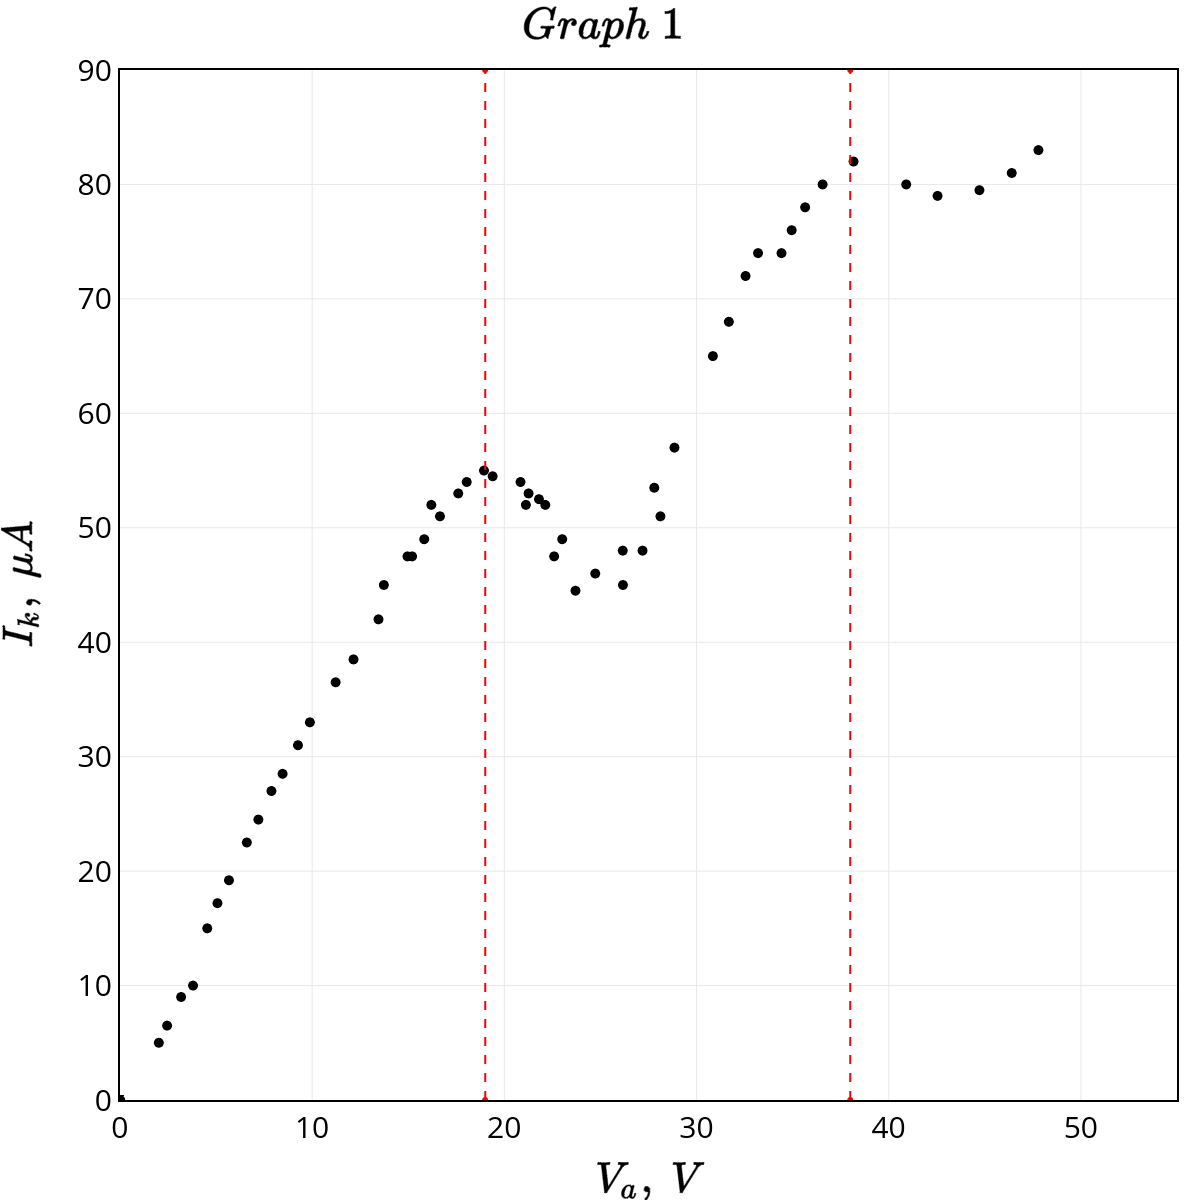
\includegraphics[scale=0.17]{my_plot1.png}}
\end{figure}

Для проверки закона Стефана-Больцмана построим в логарифмическом масштабе график зависимости 
\begin{gather*}
W = \ln(\epsilon_T B) + n\ln(T).
\end{gather*}

\begin{figure}[h]
\center{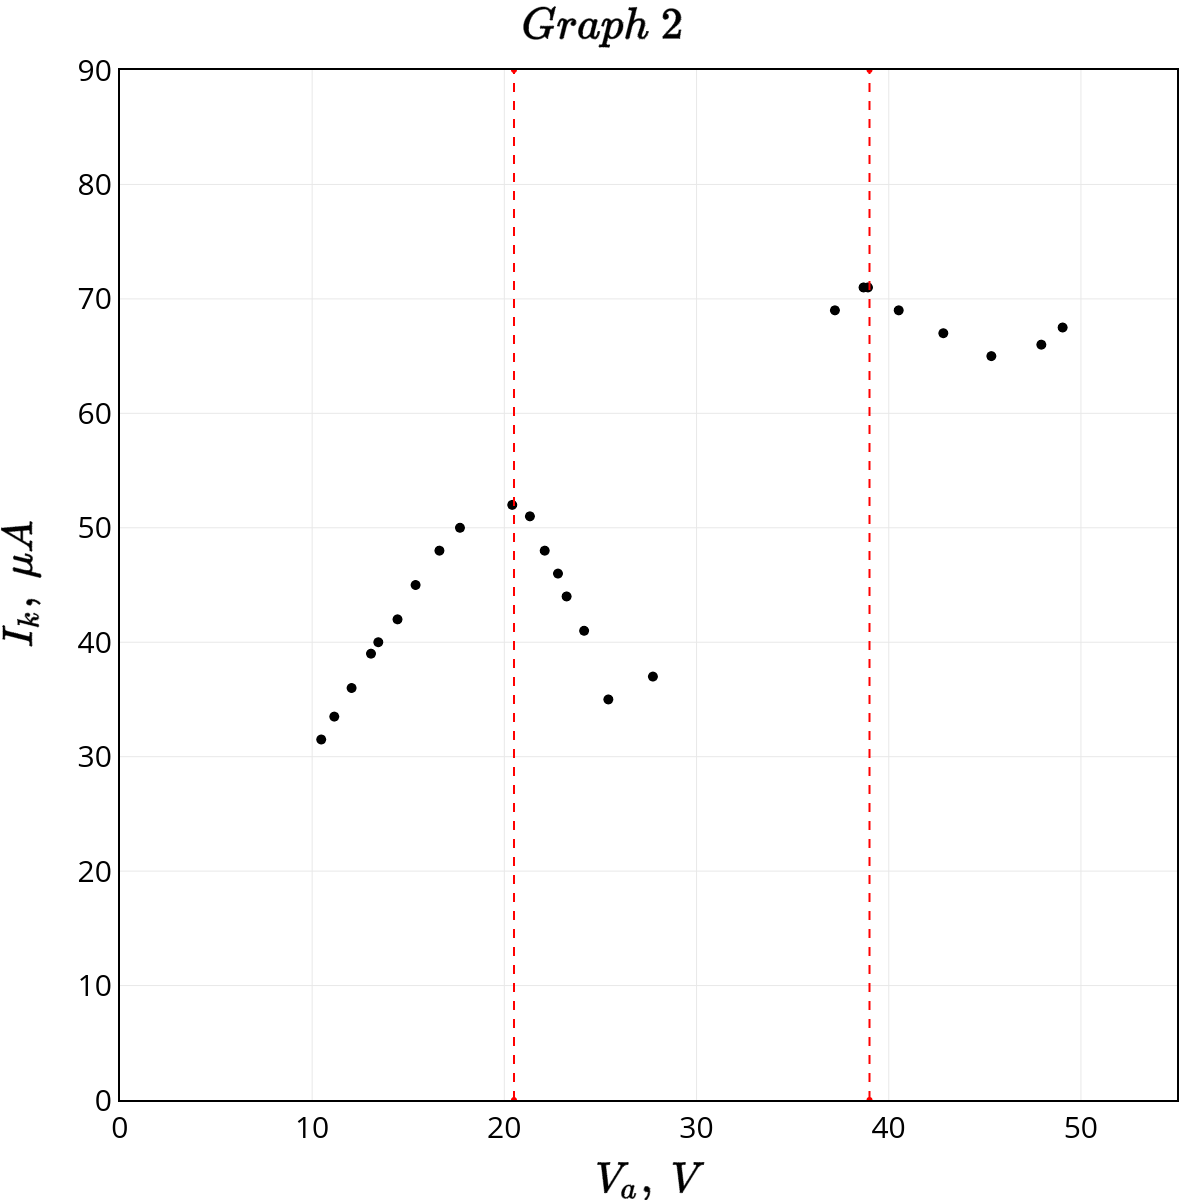
\includegraphics[scale=0.17]{my_plot2.png}}
\end{figure}

В общем случае $\epsilon_T = \epsilon_T(T)$, и так как в наших измерениях присутствуют значения температуры с шагом в $50~K$, которые не даны в табличных данных, интерполируем значения до необходимых и построим график зависимости $\epsilon_T = \epsilon_T(T)$.

\begin{figure}[h]
\center{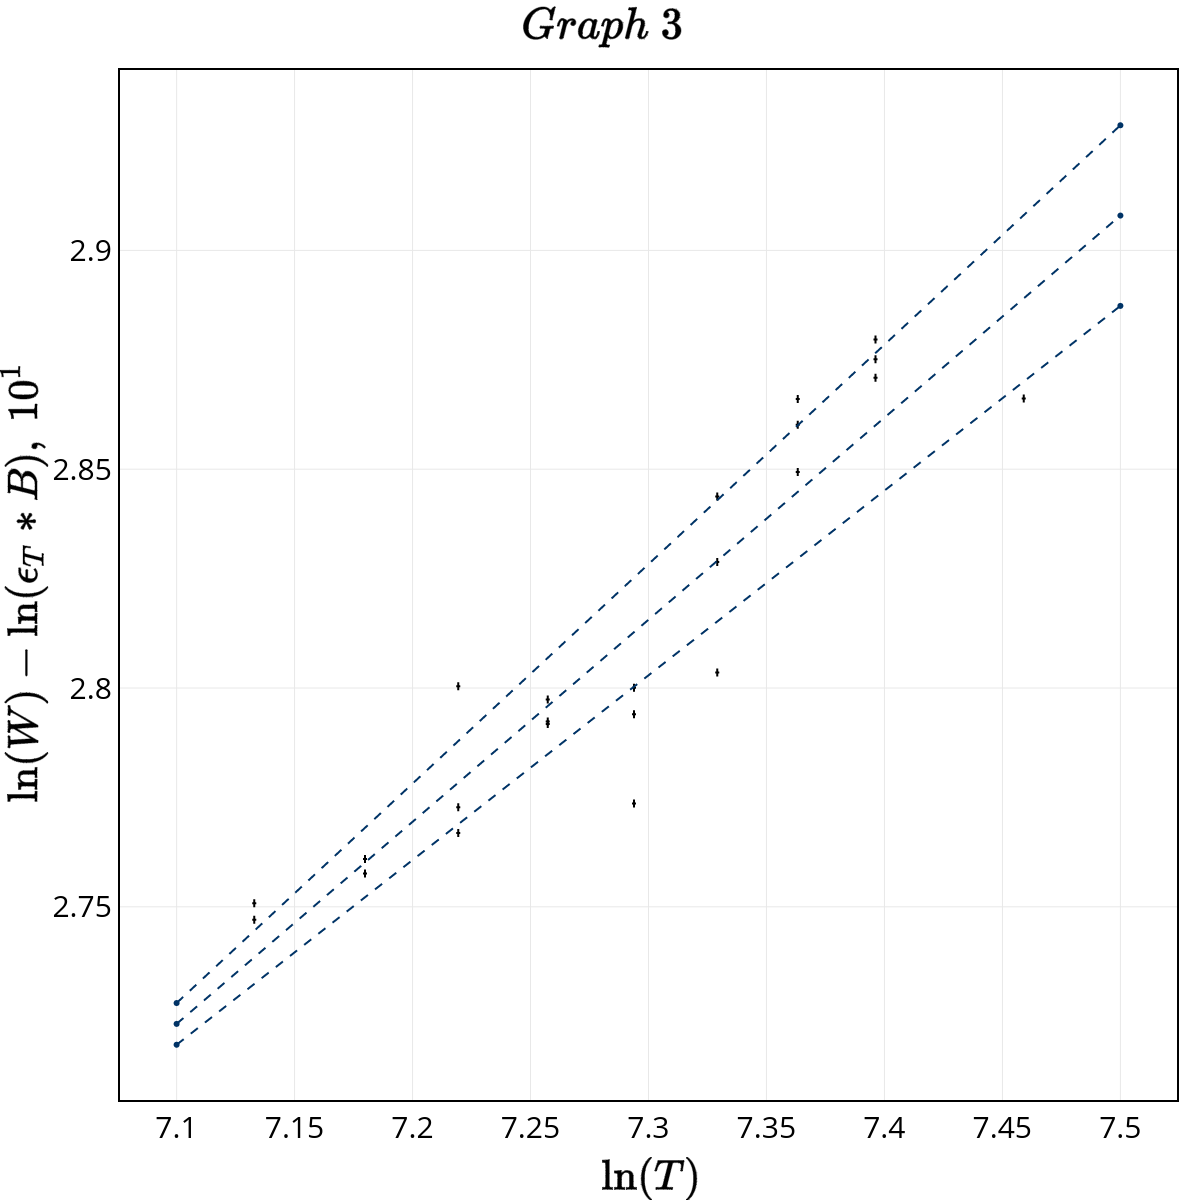
\includegraphics[scale=0.17]{my_plot3.png}}
\end{figure}

Теперь построим регрессионную модель для зависимости 
\begin{gather*}
W - \ln(\epsilon_T B) \sim \ln(T)
\end{gather*}
и получим оценку и доверительный интервал для параметра показателя степени температуры
\begin{gather*}
n = 4.6 \pm 0.4^{\text{stat}}.
\end{gather*}

Теперь найдём величину постоянной Стефана-Больцмана по формуле
\begin{gather*}
\sigma = \frac{W}{\epsilon_T S T^4}
\end{gather*}
для каждого измеренного значения $T$.

\begin{figure}[h]
\center{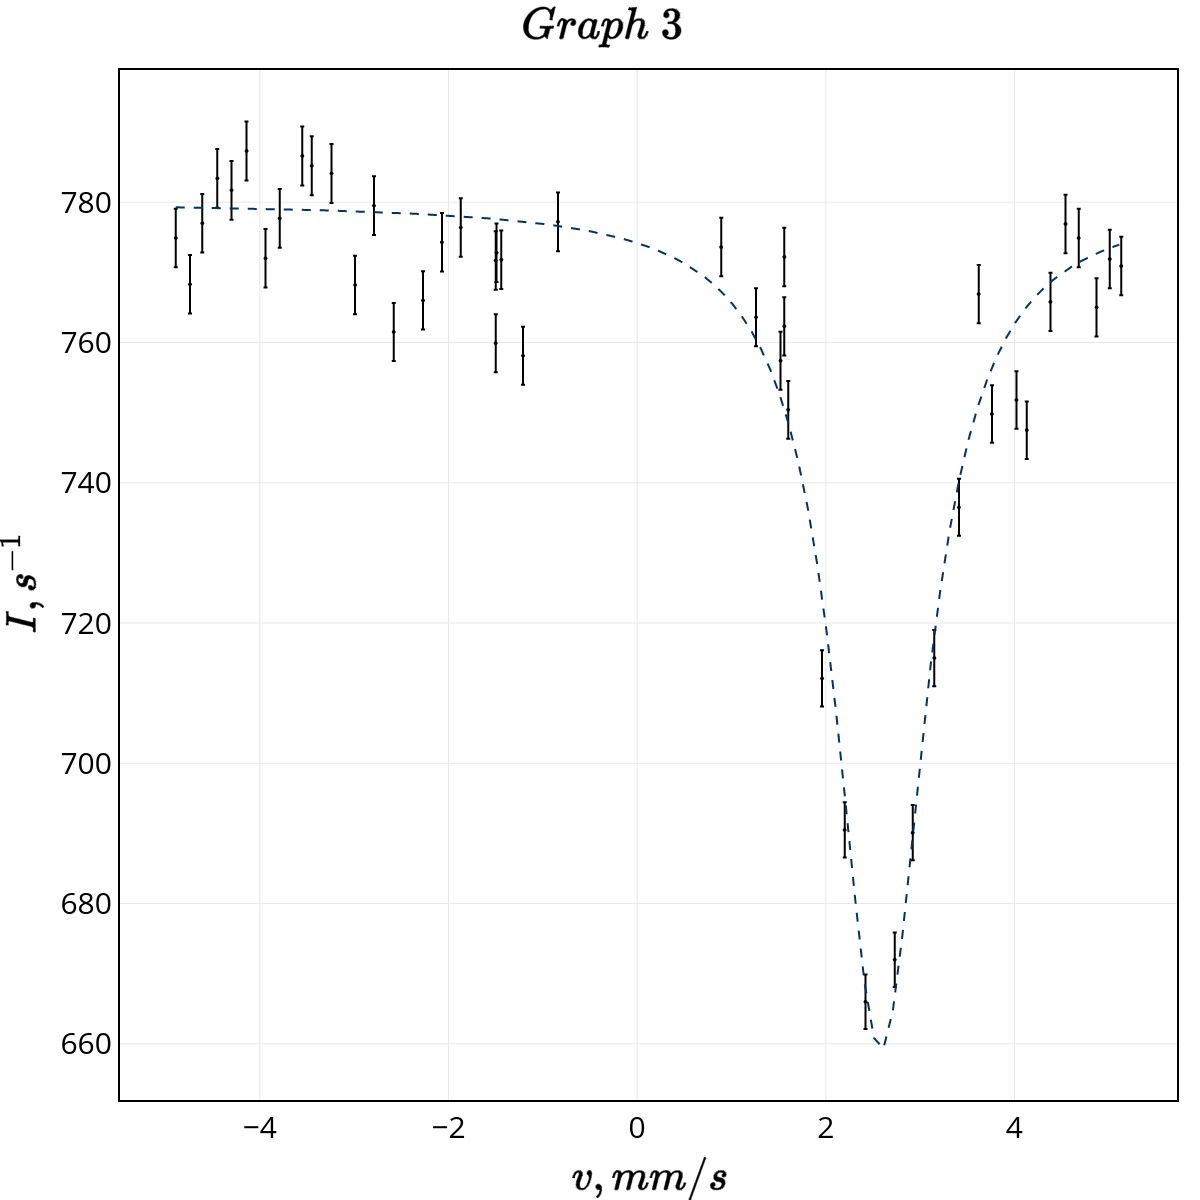
\includegraphics[scale=0.17]{my_plot4.png}}
\end{figure}

По найденным значениям $\sigma = \sigma(T)$ определим оценку и доверительный интервал для $\sigma$, как параметра, не зависящего от температуры $T$.
\begin{gather*}
\sigma = (5.4 \pm 0.1) \cdot 10^{-8}~W \cdot m^{-2} \cdot K^{-4}.
\end{gather*}

Определим величину постоянной Планка $h$, оценим точность её определения, а также сравним с табличной
\begin{gather*}
h = (6.9 \pm 0.2) \cdot 10^{-34}~J \cdot s,\\
h_{\text{табл}} = 6.62 \cdot 10^{-34}~J \cdot s.
\end{gather*}

\item
\textbf{Измерение "яркостной температуры" неоновой лампочки}\\

Направим пирометр на неоновую лампочку и измерим пирометром "яркостную температуру" неоновой лампочки. Дотронувшись до лампочки рукой, убедимся, что термодинамическая температура лампочки не соответствует измеренной яркостной температуре нагретого тела.
\begin{gather*}
T_{\text{неон}} = 1300 \pm 1^{\text{syst}}~K
\end{gather*}

Данный факт легко объяснить другим механизмом излучения отличным от механизма теплового излучения.

\end{enumerate}

\end{document}